% Created 2022-09-16 vie 12:58
% Intended LaTeX compiler: pdflatex
\documentclass[12pt]{article}
\usepackage[utf8]{inputenc}
\usepackage[T1]{fontenc}
\usepackage{graphicx}
\usepackage{grffile}
\usepackage{longtable}
\usepackage{wrapfig}
\usepackage{rotating}
\usepackage[normalem]{ulem}
\usepackage{amsmath}
\usepackage{textcomp}
\usepackage{amssymb}
\usepackage{capt-of}
\usepackage{hyperref}
\usepackage[spanish]{babel}
\usepackage{graphicx,geometry}
\geometry{ a4paper, left=1in, right=1in, top=1in, bottom=1in }
\renewcommand\familydefault{\sfdefault}
\usepackage{sectsty}
\usepackage{tabularx}
\usepackage{listings}
\lstdefinestyle{mystyle}{
numbers=left,
showspaces=false,
frame=leftline,
showspaces=false,
showstringspaces=false,
showtabs=false,
numberstyle=\tiny,
}
\lstset{
style=mystyle,
literate={á}{{\'a}}1
{é}{{\'e}}1
{í}{{\'{\i}}}1
{ó}{{\'o}}1
{ú}{{\'u}}1
{Á}{{\'A}}1
{É}{{\'E}}1
{Í}{{\'I}}1
{Ó}{{\'O}}1
{Ú}{{\'U}}1
{ü}{{\"u}}1
{Ü}{{\"U}}1
{ñ}{{\~n}}1
{Ñ}{{\~N}}1
{¿}{{?``}}1
{¡}{{!``}}1
}
\makeatletter
\usepackage{mdframed}
\BeforeBeginEnvironment{minted}{\begin{mdframed}}
\AfterEndEnvironment{minted}{\end{mdframed}}
\author{Luis Eduardo Galindo Amaya \\
1274895}
\date{2022-09-15}
\title{Esquematización de los Componentes de una \\
Interfaz de Usuario}
\hypersetup{
 pdfauthor={Luis Eduardo Galindo Amaya \\
1274895},
 pdftitle={Esquematización de los Componentes de una \\
Interfaz de Usuario},
 pdfkeywords={},
 pdfsubject={},
 pdfcreator={Emacs 26.3 (Org mode 9.1.9)}, 
 pdflang={Spanish}}
\begin{document}

\maketitle

\newcommand{\docente}{Manuel Castañón-Puga}
\newcommand{\asignatura}{Herramientas de Desarrollo de Software (40017)}
\newcommand{\semestre}{2022-2}

%\setlength\parindent{0pt}   % eliminar el intentado
\setlength{\parskip}{1.2em}


\section*{Componentes}
\label{sec:org26a1052}
\begin{center}
\begin{tabular}{ll}
Button & Un botón sirve para hacer clic y realizar una acción.\\
Checkbox & Puede representar un estado booleano estable.\\
Radiobutton & Se usan en grupos y pueden una opción de varias.\\
Combobox & Permite seleccionar un string de una lista.\\
Label & Texto en la pantalla.\\
Menubar & Barra de herramientas, da acceso rápido a comandos comunes\\
Popupmenu & Menú desplegable, puede integrar varios comandos cómodamente\\
Scollbar & Permite ver componentes de un mayor tamaño que la pantalla\\
Textarea & Permite ingresar texto de mas de una linea\\
Textfield & permite. ingresar textos de una longitud reducida\\
\end{tabular}
\end{center}

\section*{Ensayo}
\label{sec:orgfb128f6}
A lo largo de la carrera hemos creado diversos programas para realizar diversas tareas especificas, sin embargo normalmente no usamos la terminal para trabajar con nuestros programas (o al menos la mayoría de las  veces), las interfaces gráficas tienen diversos tipos de componentes que cumplen roles muy específicos para los usuarios, desde capturar texto hasta seleccionar de una lista de opciones.

Los componentes de las interfaces de usuario también pueden cumplir con el rol intermedio de validar los datos antes de pasarlos al programa como una forma de validación, por lo que elegir los tipos adecuados puede ayudar a simplificar los procesos de creación del software.

En la actualidad las interfaces de computadora dominantes son sin duda las pantallas tactiles pero poco a poco otro tipo de interfaces se van abriendo un espacio, tecnologias que procesan lenguaje natural se han vuelto bastante comunes (Amazon Alexa y Google Home), las pantallas tactiles abarcantodo los ambitos de nuestra vida cotidiana actual, desde hacer check-in en el aeropuerto, rellenar formularios en tablets, ver menus en los restaurantes sin olvidar que siempre tenemos una en el bolsillo que nos permite extender la funcioanlidad de nuestros dispositivos de la forma que mas nos sirva.

Las interfaces de usario siempre han sido sobre hacer la tecnologia mas sencilla y sin duda la manera mas sencilla es usando el cuerpo humano (total no ocupas una interfaz si tu eres la interfaz ¿no?) desde reconocimiento de lenguaje natural, captura de movimiento o incluso podria ser una interfaz cerebro-maquina que nos permita controlar las cosas con nuestro pensamiento, aunque eso seria mirar demaciado hacia el futuro.

Para concluir me gustaría hacer un párrafo sobre la modificación del cuerpo humano, una vez que los dispositivos puedan adaptarse al 100\% a nuestro requerimientos lo siguiente sera empezar a expandir nuestras capacidades, por ejemplo si ya tenemos la capacidad de controlar dispositivos con nuestros pensamientos podría ser posible que una persona que no cuente con una extremidad pueda conectarse una prótesis mecánica sin tener que recurrir a cirugía y e incluso si nuestro entendimiento del cuerpo humano es suficiente podríamos transmitir información no solo de nuestra mente al dispositivo biomecánico si no que de la prótesis al cerebro también sin tener que hacer una operación, podemos seguir expandiendo esta idea hasta que llegamos al punto que un usuario podría recrear todas sensaciones humanas sin necesidad de un cuerpo biológico y en ese punto ya no seria necesario crear mas interfaces porque podríamos extender a nuestro placer estos cuerpos no biológicos y optimizarlos para lo que nos plazca, desde trabajar en lugares peligrosos hasta estar en el vació del espacio sin necesidad de estar presencialmente allí.

\section*{Reflexion final}
\label{sec:org7b5a8cf}
Las interacciones con nuestros dispositivos son la manera en la podemos extender muestras capacidades, una transparencia entre dispositivos y nuestra forma de operarlos va mas allá de su facilidad de uso, también puede producir cambios radicales en la forma en la que vivimos, en años recientes pudimos ver la revolución de los teléfonos inteligentes la cual cambió por completo la dinámica de los transportes comunicación etc. 


\begin{center}
Doy fe de que toda la información dada es  completa y correcta. \\
\begin{center}
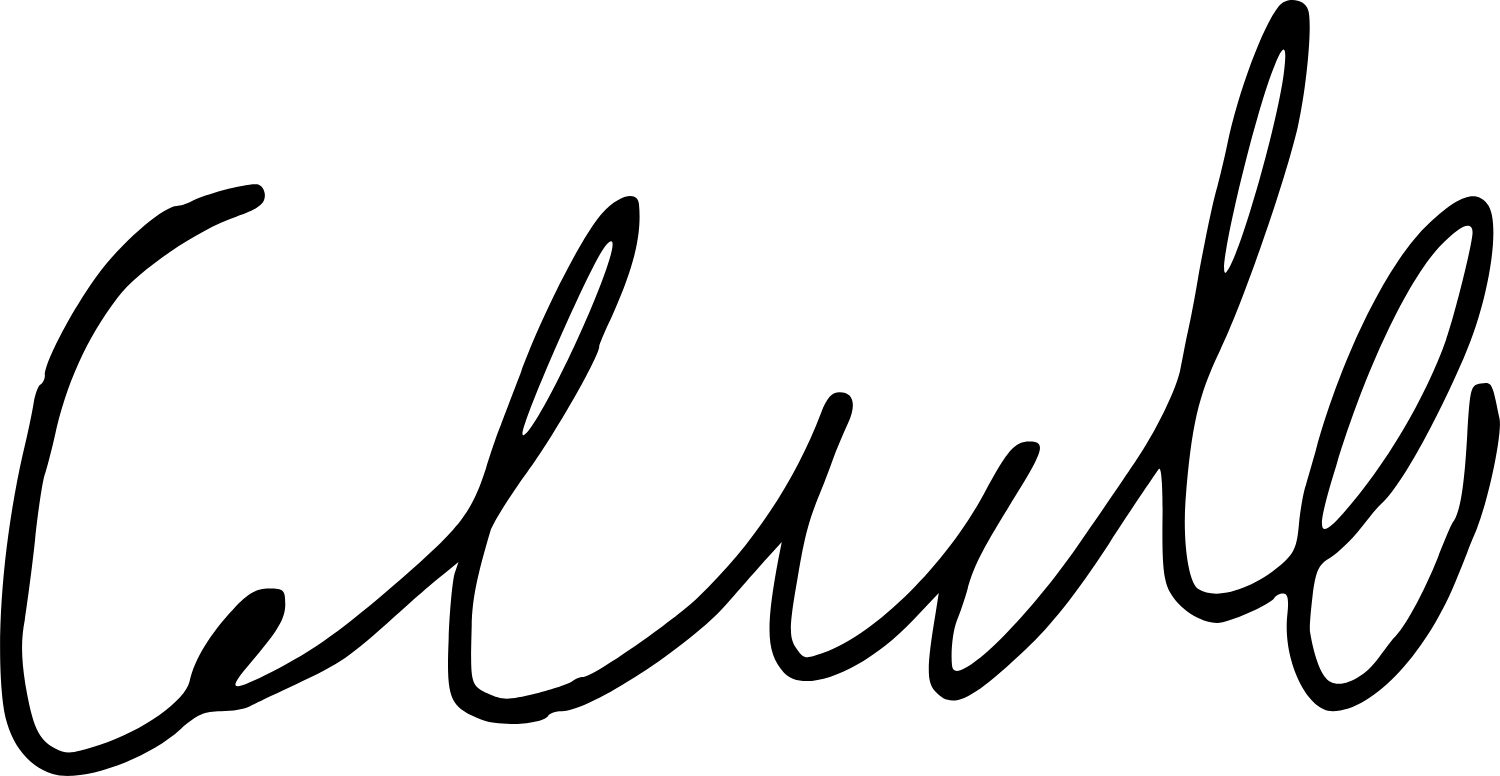
\includegraphics[width=3cm]{../includes/firma.png}
\end{center}
Luis Eduardo Galindo Amaya \\
1274895
\end{center}
\end{document}
